\documentclass[]{article}
\usepackage{amssymb}
\usepackage{amsmath}
\usepackage{booktabs}
\usepackage{graphicx}
\DeclareMathOperator*{\argmax}{arg\,max}
\DeclareMathOperator*{\argmin}{arg\,min}
\DeclareMathOperator*{\sign}{sign}

\usepackage{float}
\usepackage{newfloat}
\DeclareFloatingEnvironment[placement={!ht},name=List]{mylist}
%opening
\title{Peers Suggestion Algorithm}
\author{OakNorth Machine Learning}

\begin{document}

\maketitle

\begin{abstract}
Correctly understanding the performance of a borrower is a critical part during 
the lifetime of a loan for lenders. Without comparing with other companies, it 
is hard to defend any claim of the status of financial-health of a company. In 
this document, we describe a data-driven machine learning algorithm that 
constructs a set of companies, i.e., peers, for benchmarking a specific 
company automatically. 
\end{abstract}

\section{Introduction}

``\textit{Good}" is a relative concept. When we claim a company is financially  
good, not only we assert the intrinsic properties of this company, 
we are also claiming that the entity is performing \textit{better} than 
\textit{something}. The procedure of finding out something to be compared 
against is common during credit underwriting and monitoring in OakNorth. This 
procedure, named ``Peer Benchmarking", starts with carefully selecting a set of 
companies, and their financials are used to be compared with a company. To
have an unbiased and objective view of financial-health, selection has to be 
done with strict criteria, and some of them cannot be quantitatively measured, 
as shown below:
\begin{mylist}
    \begin{enumerate}
        \item A peer should have similar business model, same type of primary 
        revenue source. 
        \item A peer should be at similar size, debt level, profitability, 
        revenue 
        level, etc.
        \item A peer should operate under a similar jurisdiction system.
        \item A peer should not be owned by the same chain of entities.
        
    \end{enumerate}
    \caption{List of factors that are considered when analysts are 
    selecting peers.\label{list:req}}
\end{mylist}

While it is an essential part of OakNorth credit workflow, the manual process 
on 
average requires 8 analyst * working hours to complete, due to data 
discoverability, and task complexity. Second, the criteria is nebulous and hard 
to transfer to junior analysts, and this leads to additional time spent by 
senior analysts to train junior analysts and review their 
selections. As this is a bottleneck of manual workflow, OakNorth machine 
learning team has worked with credit analysts closely to derive 
a data-driven approach that reduces the time of peer selection from 8 analysts 
* hours to 30 analyst * minutes. On the one hand, the dramatic improvement of 
speed has liberated our analysts from the tedious tasks of manually reading 
lines of business descriptions to focus on more creative 
tasks that require human intelligence. On the other hand, the suggestion 
algorithm allows us to generate analytics (on top of peers) automatically on 
more cases while previously it would be impossible due to labour 
resource constraint. The remained part of this paper is split into three 
sections, 
whereas the first and second section will focus on modelling 
and annotations collection, and the third part will look into how the system 
is integrated with OakNorth Platform. 


\section{Modelling}
We model peers selection problem as a ranking problem. For a given base company 
(hereafter referred as the query company, or just query), the algorithm aims to 
score\footnote{Giving scores in real space to companies implies we can rank 
them as real space is total-ordered. We will use score and rank interchangeably 
throughout the paper.} companies in OakNorth data platform based on how likely 
they are good peers with respect to the query. 

We have adopted Learning to Rank (LTR) methodology from the seminal work from 
Microsoft \cite{burges2005learning} to obtain a good scorer with training data 
gathered from domain experts. On a high level, LTR attempts to learn whether a 
given entity is relevant for a given query based on a set of extracted features 
for the entity/query pair. These features, together with a label of the 
relevance of a given peer for a given query provide the basis for our 
training routine.

Formally, let a scorer $f$ be a function that takes 
into two arguments and return a real number, i.e. $f: C\times C \mapsto 
\mathbb{R}$, $C$ be the set of all companies. Assume we have collected 
a 
dataset consists of a set $\mathcal{Q}=\{q_i\}_{i=1}^N\subseteq C$ represents a 
set 
of queries, i.e. base companies. $D_i=\{(c_{ij}, r_{ij})\}_j$ represents a set 
of 
potential candidates for a base company $q_i$. Each element of $D_i$ 
is a tuple of a candidate company $c_{ij}\in C$ and a score 
$r_{ij}\in\mathbb{R}$ on 
how relevant $c_{ij}$ is with regards to $q_i$. A good scorer needs to return a 
higher score on relevant candidates and less so on the poorer ones, and to 
mathematically capture the \textit{fitness} of a scorer, i.e. how good it is 
with respect to the dataset we collected $\mathcal{Q}$ and $D_i$, we adopt the 
\textbf{RankNet} \cite{burges2005learning} loss. 

\begin{align}
\begin{split}
    \mathcal{L}_i &= \sum_{\substack{(c_j, r_j), (c_k, r_k)\in D_i \\ r_j < 
    r_k}}{-\log\sigma(C_{i, j, k})} \\
    C_{i, j, k} &= f(c_i, c_k) - f(c_i, c_j)
    \label{eq:loss}
%    C(c_i, c_j, c_k) &= -\log \frac{}{den}
\end{split}
\end{align}

where $\sigma$ is sigmoid function.

Intuitively, $C_{i, j, k}$ measures the unnormalised likelihood of the event 
where $c_k$ is more relevant than $c_j$ with respect to $c_i$. Sigmoid function 
normalises the measure to a probability, and $L_i$ is the negative likelihood 
of observing the ordered companies implied from the dataset $q_i$, 
$D_i$\footnote{This 
training objective does not measure fitness by how 
close the scores given by the model are to the ground-truth scores, it 
only measures the consistency of the ordering, which is considerably a much 
easier task to solve.}. Suppose the scorer is parametrised by $\theta$, i.e. 
$f_\theta$, we can find out the best model with respect to the dataset above by 
solving the following optimisation problem:

\begin{align}
\begin{split}
\theta = \argmin_\theta{\sum_i \mathcal{L}_i}
\label{eq:optimisation}
\end{split}
\end{align}

\subsection{Company Representation and Features}
Based on the intuitions from domain experts, there are 
certain fields the algorithm needs to inspect in order to judge correctly the
relatedness between two companies. As shown in 
table \ref{tab:features}, we used different metadata to capture similarities 
between two companies from different aspects. For example, the 
model relies mostly on business descriptions to infer similarity on business 
model and main source of revenue, while it uses last reported financials as a 
proxy to measure similarity of company size and profitability level. The full 
details about how we convert company meta-data into similarity can be found in 
the appendix.

We define each function that captures different aspects of similarity a 
\textit{feature 
function} (or feature in short). Some 
features in the model can be parameterised so that it can be trained, 
e.g. BERT\cite{devlin2018bert}, while some are designed with domain experts to 
capture specific nuance in the task, e.g. Company Ownerships. The output of 
every 
feature function is aggregated linearly, as follows

\begin{align}
\begin{split}
f_{\theta}(c_i, c_j) = \sum_k w_k \phi_\theta(c_i, c_j)
\end{split}
\end{align}

and $w_k\in\theta$ is trainable parameter. Under the hood, we make sure $f$ is 
differentiable with respect to all parameters $\theta$ ``almost everywhere" and 
we used stochastic gradient descent \cite{bottou2018optimization} to optimise 
the objective in equation \ref{eq:optimisation} to obtain a stationary point in 
the optimisation problem.



\begin{table}[]
    \begin{tabular}{@{}p{4cm}p{7cm}@{}}
        \toprule
        Meta-Data                                      & Features to measure 
        similarity                            \\ \midrule
        Company Description                            & TF-IDF\cite{saltonIR}, 
        BERT\cite{devlin2018bert}                                      \\
        Country of Risk                                & Parity of Countries. 
        Geolocation Proximity.               \\
        Last reported financials, e.g. EBITDA, Revenue & Parameterised 
        piece-wise constant 
        function in log-scale \\
        Company Structure                              & 
        Subsidiarity                                              \\ \bottomrule
    \end{tabular}
\caption{Meta-data used to represent companies, and features derived from 
it.            \label{tab:features}}
\end{table}

\section{Annotation}
In the last section, we derived a model by assuming the dataset $Q$ 
and $D_i$ are prepared. Yet there is a more important and fundamental question 
we need to ask: is peer suggestion task even learnable? Imagine a scenario 
where there is a room filled with domain experts. Half of the group always 
make contradictory judgements to another half about whether a company is peer 
or not. Regardless of how good a scorer is, it cannot convince more than 
half of the domain experts in the room. In other words, if the agreement, i.e. 
consensus is low, we will not be able to produce any convincing system to 
automate this task.

\subsection{Consensus}
We conducted an experiment to understand consensus: if different 
analysts are asked the same question about peers, would similar decisions be 
made? If we were to examine consensus of such decisions which are made in a 
real-world environment, the consensus level would likely be low as there are 
overwhelmingly many exogenous variables to affect the decisions. To produce 
meaningful result, we have to appropriately constrain the environment to 
improve agreement. 

We start by looking at a typical workflow of manual peer selection, which 
consists of \textbf{1)} based on criteria in list \ref{list:req}, 
e.g. sector type, total revenue, geo-location, etc., short-list a set of 
candidates, \textbf{2)} with the set of candidates, refine the results with 
external information, e.g. Google, Bloomberg, Capital IQ, etc.

We focus our effort on the first phase of the task, and, by providing a good 
set of good initial candidates, we can reduce the time analysts spend on phase 
2. Accordingly, the consensus experiments will be constrained in the following 
way. Each annotator will receive a list of base companies, and 20 companies 
suggested by baseline \footnote{The first baseline is the default ranker in 
Elastic Search \cite{es}.} in an excel sheet with each base company. Each 
annotator is asked to:
\begin{mylist}[H]
    \begin{enumerate}
        \item Label each suggestion as positive, which means the suggested 
        company is a potentially good company to benchmark the base borrower, 
        or negative vice versa.
        
        \item If the company is marked as positive, annotate relatedness with 
        three levels: most relevant, relevant, and least relevant.
        
        \item Factor in financials availability in relatedness 
        judgement, instead of positivity judgement. 
        
        \item Each annotator can only answer the question with information from 
        the excel sheet, (i.e. OakNorth Platform). They cannot annotate with 
        external information such as Google, or Bloomberg Terminal.
        
        \item Each annotator cannot share any information among each other 
        during the experiment.
        
    \end{enumerate}
\caption{The specification of the annotation task.\label{list:annotation}}
\end{mylist}

We have collected 1500 judgements from 6 different analysts, and we 
examine the inter-annotator agreement regarding positivity of peer candidates. 
The agreement is over 75\% which is high compared to other tasks in Machine 
Learning \cite{mozetivc2016multilingual,nowak2010reliable}. This also defines a 
natural upper bound of performance for the task.

\subsection{Training}

Some reader may have noticed the similarity of the form of annotations in list 
\ref{list:annotation} and the notations in equation \ref{eq:loss}. 
Specifically, each base company forms $q_i$, the 20 suggestions are $c_{i, j}$ 
and the positivity and relatedness judgement are $r_{i, j}$. We map 
``negative", ``less relevant", ``relevant", and ``most relevant" to real 
numbers 0, 1, 2, and 3. Plugging everything together, we can train the models 
with the annotations gathered and equation \ref{eq:optimisation}.

\section{Integration}
The end-to-end pipeline of peer suggestion system consists of three 
parts. \textbf{1)} An Extract-Transform-Load(ETL) pipeline that prepares, 
cleans and index the dataset we gather from external data vendors, such as 
Capita IQ, Orbis and Factset into an Elastic Search system. \textbf{2)} From 
millions of companies, peers system uses a set of high-recall heuristics, 
detailed in the appendix, to 
shortlist hundreds of candidates from Elastic Search. \textbf{3)} The machine 
learning ranker will 
rank hundreds of candidates and pick out the 20 most relevant ones to present 
to the platform. 

\begin{figure}[h]
    \centering
    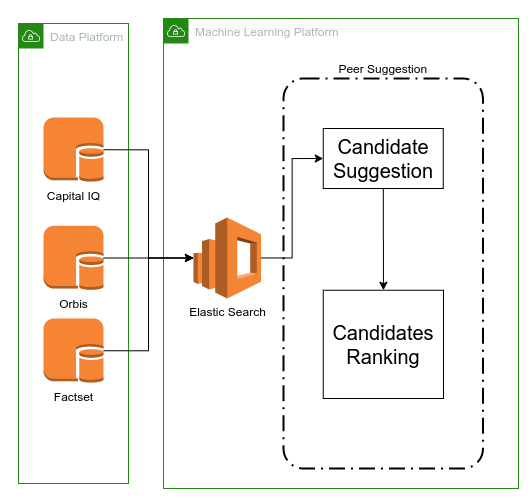
\includegraphics[width=.95\linewidth]{./fig/peers.png}
    \caption{Elastic Search index in ML platform indexes the aggregated and 
    properly consolidated dataset. We use a set of high recall heuristics to 
    select the most promising candidates, then the data-driven model ranks the 
    candidates and present the best 20 suggestions to the 
    platform.\label{fig:peers_integration}}
\end{figure}

\bibliographystyle{unsrt}
\bibliography{main.bib}

\appendix
\section{Details of Features}
Based on different fields in the company meta-data, we derive different 
functions to measure similarity from different aspects. 

\subsection{Company Description}
We used unigram and bigram 
term-frequency-inverse-document-frequency (tf-idf)\cite{saltonIR} to measure 
the difference between two companies by their descriptions. In particular 
cosine distance of the tf-idf representations of two company 
descriptions is used. The document frequency table is built by all company 
descriptions in OakNorth Data Platform.

Besides, we use BERT\cite{devlin2018bert} representation to capture subtle 
semantic differences on the business descriptions. We used the pooled hidden 
status in the last layer from BERT to represent company description and use the 
dot product to capture similarity.

\subsection{Country of Risk}
We have a feature that outputs 1 when two companies have the same country of 
risk, and 0 otherwise. 

We have a feature that outputs 1 when two companies are in the same economic 
region and 0 otherwise.

\subsection{Last Reported Financials}
In words, the intuition from analysts about how they perceive financial 
similarity can be 
summarised as \textbf{1)} they look at ratios (instead of absolute difference), 
\textbf{2)} the feeling of financial similarity differs significantly from 
$\frac{f_p}{f_b}=10$ to $\frac{f_p}{f_b}=100$, but not so 
much from $\frac{f_p}{f_b}=10$ to $\frac{f_p}{f_b}=20$. \textbf{3)} the 
difference should be symmetry.

With that, we have defined a parameterised piece-wise constant function in 
log-scale to capture how analysts perception.

\begin{align}
\begin{split}
    d(f_p, f_b) = \begin{cases}
        \sum_i \mathbb{I}(b_{i-1} \leq \log_{10}(\max(\frac{f_p}{f_b}, 
        \frac{f_b}{f_p})) < b_i)c_i, & 
        \text{if} 
        \sign{(f_b)} = \sign{(f_p)} \\
        c, &\text{otherwise} 
    \end{cases}
\end{split}
\end{align}

Where $f_b$ and $f_p$ are the corresponding last-reported financials from two 
companies, 
$\{b_i\}_i, b_i\in\mathbb{R}$ is a monotonically increasing series that 
starts with 0, i.e. $b_0=0$. 
$\mathbb{I}$ is conditional function that is 1 when the condition is true, and 
0 
otherwise.

Without loss of generality, assumes $f_p > f_b$ and they have the same sign, 
this function measures how much similarity score between 
$f_p$ and $f_b$ one should give, if, in log-scale, their difference is in the 
range between $b_{i-1}$ and $b_i$, we assign a score $c_i$. To make the whole 
pipeline differentiable, we hand-set $\{b_i\}_i$ to $0.0, 0.2, 0.4, 0.6, 0.8, 
1.0, 
1.2, 
1.4, 1.6, 1.8, 2.0$\footnote{One can also parametrise the conditional function 
to be a sigmoid function so that it is a soft conditional. This will make the 
training objective in equation \ref{eq:loss} differentiable with respect to 
$b_i$. This is listed as a future research item.}, and train $c_i$ and $c$ by 
data 
so that the 
model learns automatically how to quantify similarity on financials perceived 
among analysts. Each type of line-item will have an independent piece-wise 
constant function. 

\subsection{Subsidiarity}

Company description often contains useful information to infer whether a 
company is operated under a specific chain of entities. We use a named entity 
recognition system  with dependency parsing \cite{spacy2} to recognise this 
relationship. If two companies are related we will have a feature function 
returns 1, and 0 otherwise.

\subsection{Candidate Suggestion Heuristics}

We have adopted a set of high-recall heuristics to exclude the most obvious 
negatives. The set of rules are:

\begin{mylist}
    \begin{enumerate}
        \item Business descriptions of the candidate has to match part-of the 
        one of base company.
        \item The peers revenue and EBITDA must be available, and the last 
        reported financials are not older than 5 years.
        \item The regions of incorporation are the same.
    \end{enumerate}
\end{mylist}

\end{document}


